\documentclass[tikz,crop]{standalone}

\usepackage{tikz}
\usetikzlibrary{arrows,calc,shapes.geometric, backgrounds, positioning}

\pgfdeclarelayer{background}
\pgfdeclarelayer{foreground}
\pgfsetlayers{background,main,foreground}

\tikzstyle{block} = [rectangle, draw, thick, fill=blue!25, text width=5em, text badly centered, rounded corners, minimum height=4em]
\tikzstyle{mqtt} = [circle, draw, thick, fill=orange!25, text width=5em, text badly centered]
\tikzstyle{line} = [draw, ultra thick, -latex]

\begin{document}
    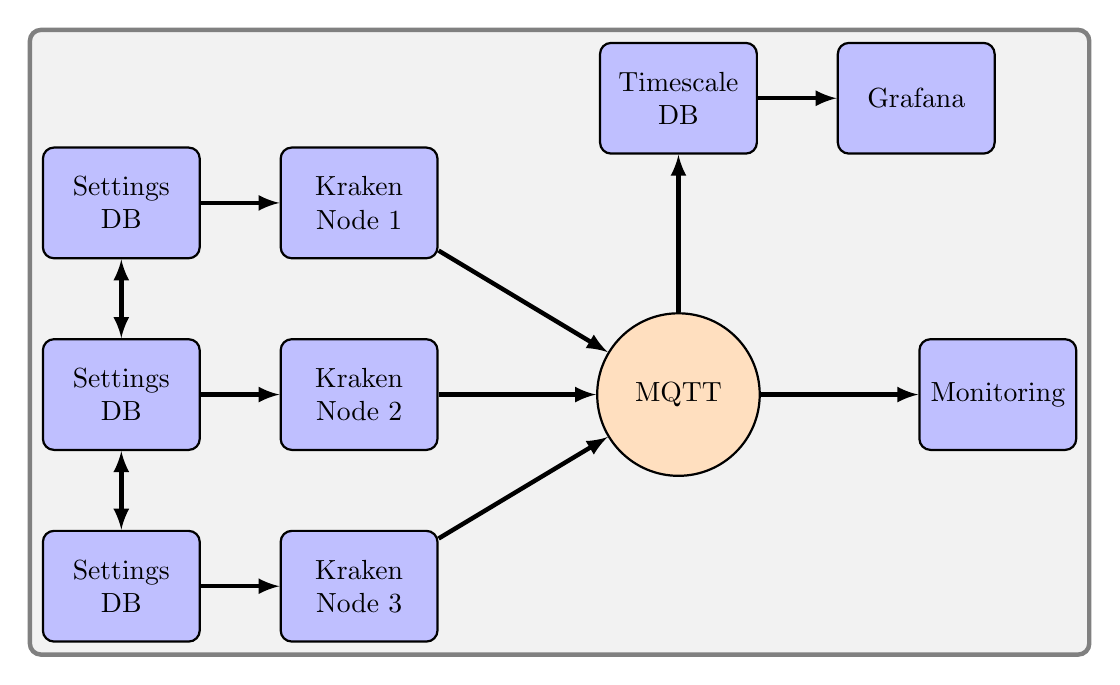
\begin{tikzpicture}[%
        node distance=1cm and 1cm,%
        auto,%
        background rectangle/.style={fill=gray!10, rounded corners, ultra thick,draw=gray},%
        show background rectangle,%
    ]
        \node[block]  (kraken)  {Kraken Node 2};
        \node[block, above=of kraken]  (kraken2)  {Kraken Node 1};
        \node[block, below=of kraken]  (kraken3)  {Kraken Node 3};
        \node[block, left=of kraken] (settings) {Settings DB};
        \node[block, left=of kraken2] (settings2) {Settings DB};
        \node[block, left=of kraken3] (settings3) {Settings DB};
        \node[mqtt, right=2cm of kraken]  (mqtt)  {MQTT};
        \node[block, above=2cm of mqtt] (timescale) {Timescale DB};
        \node[block, right=2cm of mqtt] (monitoring) {Monitoring};
        \node[block, right=of timescale] (grafana) {Grafana};
        \path [line] (settings) -- (kraken);
        \path [line] (settings2) -- (kraken2);
        \path [line] (settings3) -- (kraken3);
        \path [line] (kraken) -- (mqtt);
        \path [line] (kraken2) -- (mqtt);
        \path [line] (kraken3) -- (mqtt);
        \path [line] (mqtt) -- (timescale);
        \path [line] (mqtt) -- (monitoring);
        \path [line] (timescale) -- (grafana);
        \path [line, , latex-latex] (settings) -- (settings2);
        \path [line, , latex-latex] (settings) -- (settings3);
        % Arrows
        %\path [line] (zero) -- (calculate);
        %\path [line,rounded corners] (calculate) |- ($(calculate.south east) + (0.5,-0.5)$) |- (signal);
    \end{tikzpicture}
\end{document}
